\documentclass[aspectratio=169, 12pt]{beamer}

% ── Theme & Colors ──────────────────────────────────────────
\usetheme{default}
\usecolortheme{default}

% Custom dark color palette
\definecolor{bgDark}{HTML}{1a1a2e}
\definecolor{bgMid}{HTML}{16213e}
\definecolor{accentBlue}{HTML}{0f3460}
\definecolor{accentCyan}{HTML}{53c0f0}
\definecolor{accentGreen}{HTML}{2ecc71}
\definecolor{accentRed}{HTML}{e74c3c}
\definecolor{accentOrange}{HTML}{f39c12}
\definecolor{textLight}{HTML}{ecf0f1}
\definecolor{textMuted}{HTML}{95a5a6}
\definecolor{cardBg}{HTML}{222244}

\setbeamercolor{background canvas}{bg=bgDark}
\setbeamercolor{normal text}{fg=textLight}
\setbeamercolor{frametitle}{fg=accentCyan, bg=bgMid}
\setbeamercolor{title}{fg=accentCyan}
\setbeamercolor{subtitle}{fg=textMuted}
\setbeamercolor{author}{fg=textLight}
\setbeamercolor{date}{fg=textMuted}
\setbeamercolor{item}{fg=accentCyan}
\setbeamercolor{subitem}{fg=accentGreen}
\setbeamercolor{block title}{fg=bgDark, bg=accentCyan}
\setbeamercolor{block body}{fg=textLight, bg=cardBg}
\setbeamercolor{block title alerted}{fg=white, bg=accentRed}
\setbeamercolor{block body alerted}{fg=textLight, bg=cardBg}
\setbeamercolor{block title example}{fg=bgDark, bg=accentGreen}
\setbeamercolor{block body example}{fg=textLight, bg=cardBg}

% Fonts
\setbeamerfont{frametitle}{size=\Large, series=\bfseries}
\setbeamerfont{title}{size=\huge, series=\bfseries}
\setbeamerfont{subtitle}{size=\large}

% Remove navigation symbols
\setbeamertemplate{navigation symbols}{}

% Slide number in bottom right
\setbeamertemplate{footline}{%
  \hfill\usebeamercolor[fg]{textMuted}\scriptsize\insertframenumber{}/\inserttotalframenumber\hspace*{6pt}\vspace{4pt}%
}

% Bullet styling
\setbeamertemplate{itemize item}{\color{accentCyan}\scriptsize$\blacktriangleright$}
\setbeamertemplate{itemize subitem}{\color{accentGreen}\scriptsize$\circ$}

\usepackage{graphicx}
\usepackage{booktabs}
\usepackage{caption}
\usepackage{subcaption}
\captionsetup[subfigure]{labelformat=empty, font={color=textLight,scriptsize}}

% ── Document ────────────────────────────────────────────────
\begin{document}

% ============================================================
%  TITLE SLIDE
% ============================================================
{
\setbeamertemplate{footline}{}
\begin{frame}[plain]
\vfill
\centering
{\usebeamerfont{title}\usebeamercolor[fg]{title} Multi-Faceted Spam Email Detection\\[4pt]}
{\usebeamerfont{subtitle}\usebeamercolor[fg]{subtitle} A Comparative Study Using TF-IDF, Word2Vec \& Structural Metadata}

\vspace{18pt}
{\small\color{textLight}
Nathan Xie $\cdot$ Vijwal Akula $\cdot$ Kangyi Jiang $\cdot$ Zaid Khan Mohammed $\cdot$ Brian Cochran}

\vspace{6pt}
{\footnotesize\color{textMuted} CS 410 --- University of Illinois Urbana--Champaign --- Spring 2026}
\vfill
\end{frame}
}

% ============================================================
%  PERSON 1 — The Problem
% ============================================================
\begin{frame}{The Problem: Domain Shift}
\begin{columns}[T]
\column{0.55\textwidth}
\begin{itemize}
    \item Trained on \textbf{TREC 2007} corporate emails
    \item Tested on \textbf{SpamAssassin} public internet traffic
    \item Milestone result: \textcolor{accentRed}{\textbf{0.00 recall}} on spam class
\end{itemize}

\vspace{10pt}
\begin{alertblock}{Why?}
Different domains use entirely different vocabularies. A model that memorizes ``Enron jargon'' sees zero overlap with phishing emails in the wild.
\end{alertblock}

\column{0.42\textwidth}
\begin{block}{Feature Sparsity}
\centering
\vspace{4pt}
\small
Training vocabulary\\
$\cap$\\
Testing vocabulary\\
$\approx$ \textcolor{accentRed}{\textbf{empty}}
\vspace{4pt}
\end{block}

\vspace{8pt}
\begin{exampleblock}{Our Goal}
\small Evolve from a brittle keyword matcher into a \textbf{structurally aware}, generalizable detection engine.
\end{exampleblock}
\end{columns}
\end{frame}

% ============================================================
%  PERSON 1 — Our Approach
% ============================================================
\begin{frame}{Our Approach: Five Comparative Models}
\centering
\vspace{-4pt}
{\small\color{textMuted} Progression from simple to sophisticated feature representations}

\vspace{12pt}
\begin{columns}[T]
\column{0.19\textwidth}
\centering
\textcolor{accentCyan}{\textbf{1}}\\[4pt]
{\small Keyword\\Baseline}\\[4pt]
{\scriptsize\color{textMuted} CountVectorizer\\Unigrams only}

\column{0.19\textwidth}
\centering
\textcolor{accentCyan}{\textbf{2}}\\[4pt]
{\small TF-IDF\\Unigram}\\[4pt]
{\scriptsize\color{textMuted} IDF weighting\\No structure}

\column{0.19\textwidth}
\centering
\textcolor{accentCyan}{\textbf{3}}\\[4pt]
{\small Logistic Reg.\\Bigram+Struct}\\[4pt]
{\scriptsize\color{textMuted} TF-IDF (1,2)\\+21 features}

\column{0.19\textwidth}
\centering
\textcolor{accentCyan}{\textbf{4}}\\[4pt]
{\small Linear SVM\\Bigram+Struct}\\[4pt]
{\scriptsize\color{textMuted} Max-margin\\+21 features}

\column{0.19\textwidth}
\centering
\textcolor{accentGreen}{\textbf{5}}\\[4pt]
{\small\textcolor{accentGreen}{Word2Vec}\\+Structural}\\[4pt]
{\scriptsize\color{textMuted} Dense 50-d\\+21 features}
\end{columns}

\vspace{16pt}
\textcolor{textMuted}{\rule{0.8\textwidth}{0.4pt}}
\vspace{6pt}

{\small Each model adds one new concept $\rightarrow$ isolates its contribution}
\end{frame}

% ============================================================
%  PERSON 2 — Data Pipeline
% ============================================================
\begin{frame}{Data Pipeline \& Preprocessing}
\begin{columns}[T]
\column{0.5\textwidth}
\begin{block}{Datasets}
\begin{itemize}
    \item \textbf{Train:} TREC 2007 --- 32,091 emails\\
          {\scriptsize (12,448 ham / 19,643 spam)}
    \item \textbf{Test:} SpamAssassin --- 3,784 emails\\
          {\scriptsize (2,472 ham / 1,312 spam)}
    \item Cross-corpus = real-world OOD evaluation
\end{itemize}
\end{block}

\column{0.48\textwidth}
\begin{block}{Preprocessing Pipeline}
\begin{enumerate}
    \item \textbf{MIME Parsing} --- recursive \texttt{\_extract\_body}; plain text $\rightarrow$ HTML fallback
    \item \textbf{HTML Stripping} --- regex tag removal
    \item \textbf{URL Normalization} --- replaced with ``URL'' token
    \item \textbf{Lemmatization} --- NLTK WordNetLemmatizer
    \item \textbf{Stop Word Removal} --- via Scikit-learn
\end{enumerate}
\end{block}
\end{columns}
\end{frame}

% ============================================================
%  PERSON 2 — EDA
% ============================================================
\begin{frame}{Exploratory Data Analysis}
\begin{columns}[c]
\column{0.48\textwidth}
\centering
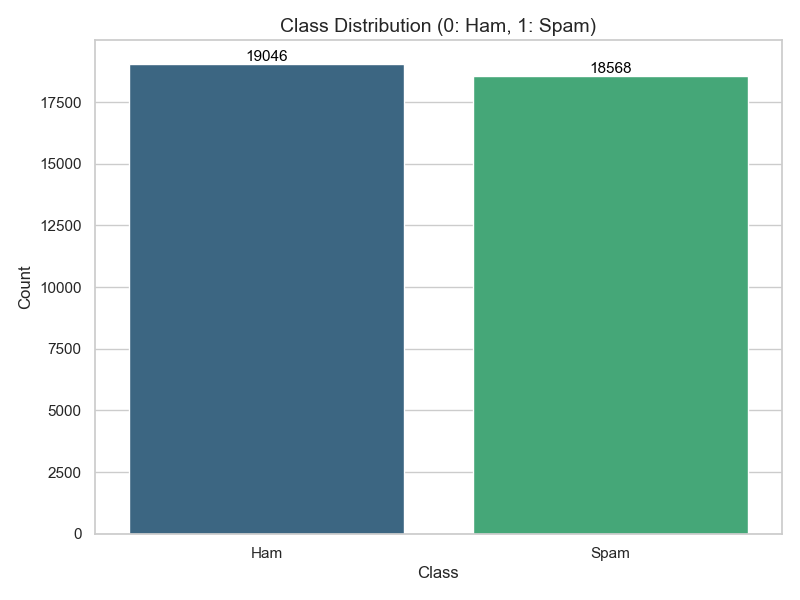
\includegraphics[width=\textwidth]{outputs/class_distribution.png}
{\scriptsize\color{textMuted} Class balance across combined corpus}

\column{0.48\textwidth}
\centering
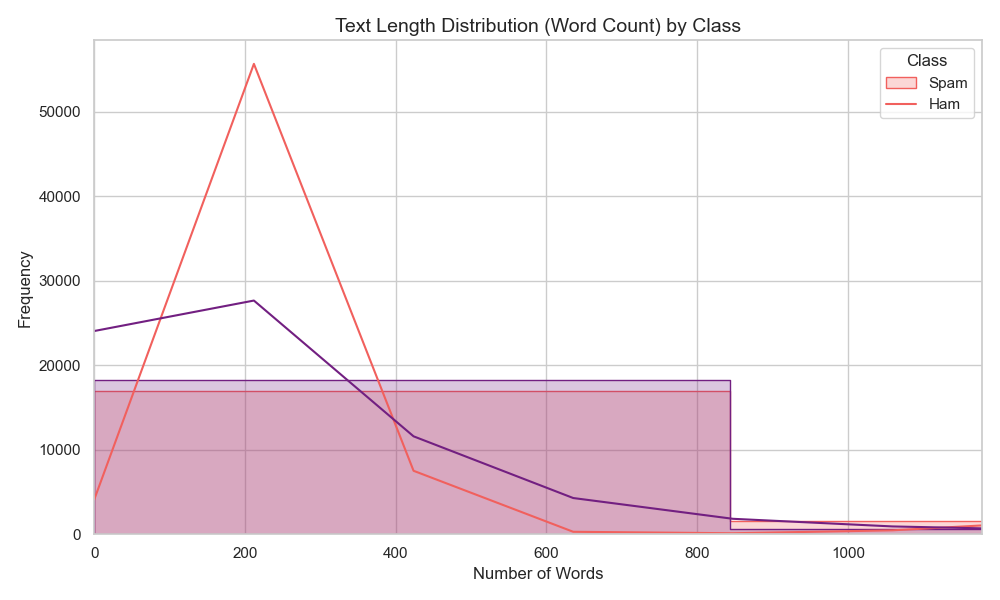
\includegraphics[width=\textwidth]{outputs/text_lengths.png}
{\scriptsize\color{textMuted} Spam concentrates at short lengths\\(automated templates)}
\end{columns}
\end{frame}

% ============================================================
%  PERSON 3 — Structural Features
% ============================================================
\begin{frame}{Structural Feature Engineering --- 21 Features}
\begin{columns}[T]
\column{0.55\textwidth}
\begin{block}{Email ``Shape'' Analysis}
\begin{itemize}
    \item \textbf{URL Density} --- hyperlinks / word count
    \item \textbf{Punctuation Intensity} --- \texttt{!} and \texttt{?} counts
    \item \textbf{Capitalization Ratios} --- all-caps ``shouting''
    \item \textbf{Sender Domain Patterns} --- validity checks, digit ratios
    \item \textbf{HTML Markers} --- content-type indicators
    \item \textbf{Length Features} --- subject, body, sender char/word counts
\end{itemize}
\end{block}

\column{0.42\textwidth}
\begin{exampleblock}{Key Insight}
\small Spam has a \textbf{distinct structural fingerprint} independent of vocabulary.

\vspace{6pt}
These 21 features persist across domains --- even when words are completely different.
\end{exampleblock}

\vspace{6pt}
{\scriptsize\color{textMuted}
Concatenated via \texttt{ColumnTransformer}\\
Normalized via \texttt{StandardScaler}}
\end{columns}
\end{frame}

% ============================================================
%  PERSON 3 — Lexical Analysis
% ============================================================
\begin{frame}{Lexical Analysis: Ham vs.\ Spam Vocabulary}
\begin{columns}[c]
\column{0.48\textwidth}
\centering
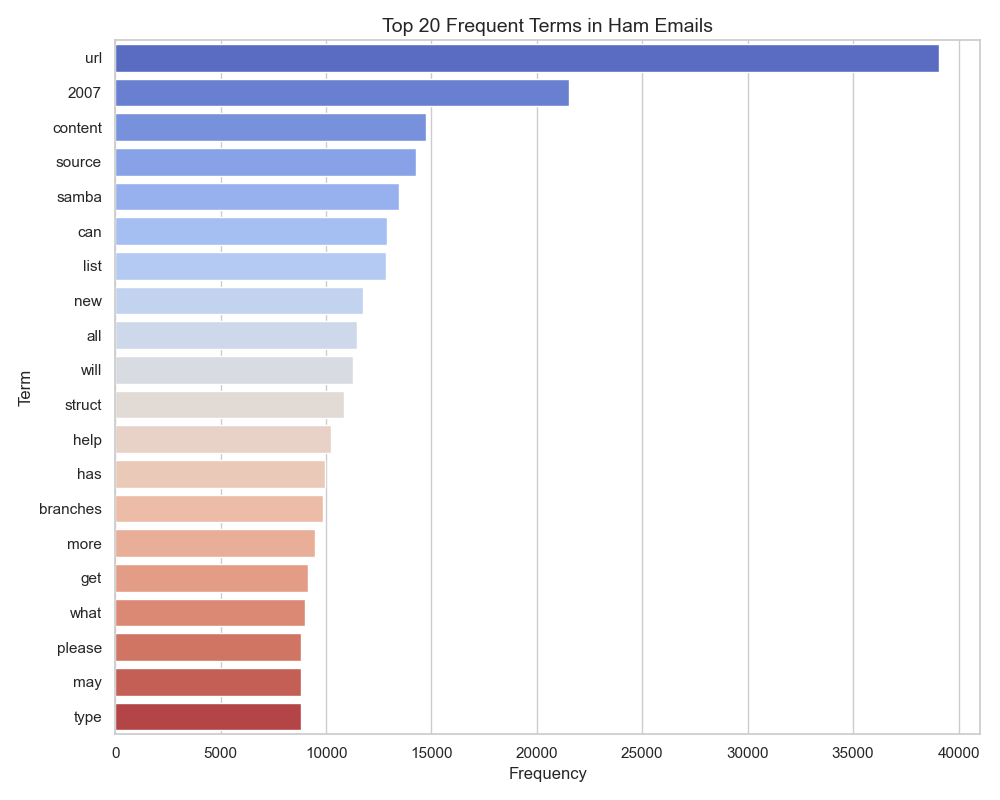
\includegraphics[width=\textwidth]{outputs/top_terms_ham.png}

\column{0.48\textwidth}
\centering
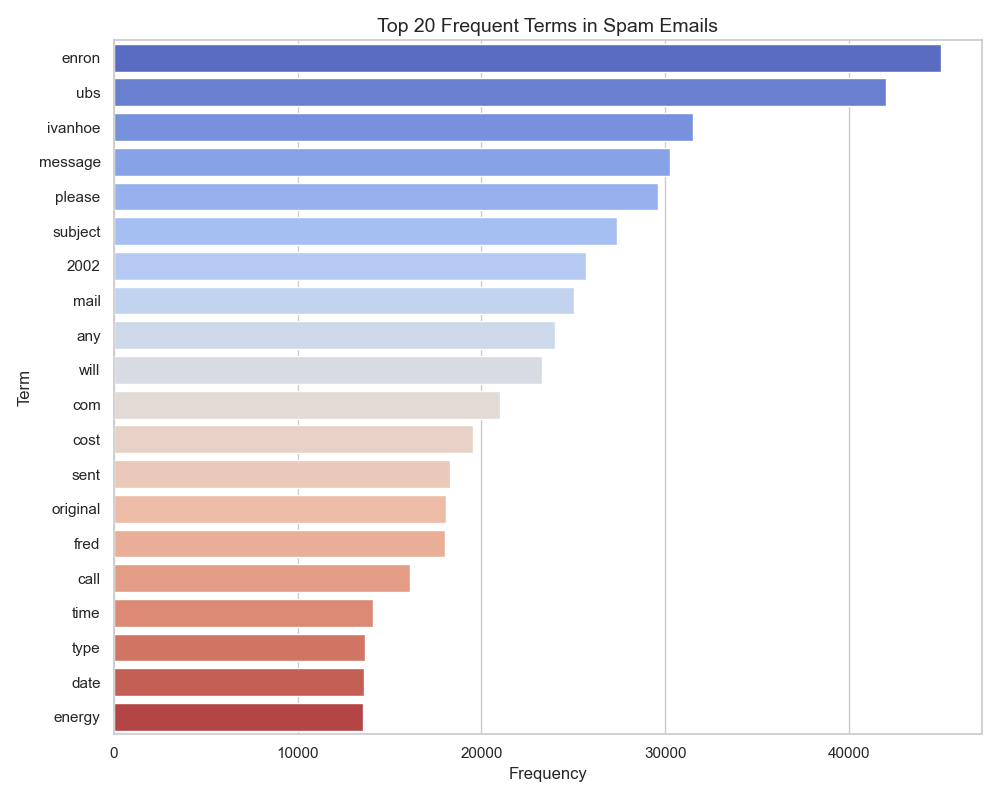
\includegraphics[width=\textwidth]{outputs/top_terms_spam.png}
\end{columns}

\vspace{4pt}
\centering
{\small\color{textMuted} Different vocabularies confirm the need for domain-invariant features}
\end{frame}

% ============================================================
%  PERSON 4 — TF-IDF Models
% ============================================================
\begin{frame}{Modeling: TF-IDF Family}
\begin{columns}[T]
\column{0.48\textwidth}
\begin{block}{Vectorization}
\begin{itemize}
    \item \texttt{TfidfVectorizer} with \texttt{max\_features=5000}
    \item Unigrams \texttt{(1,1)} vs.\ Bigrams \texttt{(1,2)}
    \item Bigrams capture phrases like\\``claim now'', ``bank account''
\end{itemize}
\end{block}

\vspace{4pt}
\begin{block}{Classifiers}
\begin{itemize}
    \item \textbf{Logistic Regression}\\{\scriptsize Probabilistic output, baseline enhanced model}
    \item \textbf{Linear SVM (LinearSVC)}\\{\scriptsize Maximum-margin hyperplane, robust to high-dimensional noise}
\end{itemize}
\end{block}

\column{0.48\textwidth}
\begin{block}{Pipeline Architecture}
\centering
\vspace{4pt}
{\small
\texttt{text} $\xrightarrow{\text{TF-IDF}}$ sparse matrix\\[6pt]
\texttt{+}\\[6pt]
\texttt{21 features} $\xrightarrow{\text{Scaler}}$ normalized\\[6pt]
$\downarrow$\\[6pt]
\texttt{ColumnTransformer}\\[6pt]
$\downarrow$\\[6pt]
\texttt{Classifier}
}
\vspace{4pt}
\end{block}

\vspace{4pt}
{\scriptsize\color{textMuted} 5-fold cross-validation on training set\\All models: F1 $> 0.99$ in-domain}
\end{columns}
\end{frame}

% ============================================================
%  PERSON 4 — Word2Vec
% ============================================================
\begin{frame}{Modeling: Word2Vec Neural Embeddings}
\begin{columns}[T]
\column{0.52\textwidth}
\begin{block}{How It Works}
\begin{enumerate}
    \item Train \textbf{CBOW Word2Vec} on corpus (Gensim)
    \item Each word $\rightarrow$ dense 50-d vector
    \item Document = \textbf{mean centroid} of word vectors
    \item Concatenate with 21 structural features
    \item Classify with \textbf{balanced} Logistic Regression
\end{enumerate}
\end{block}

\column{0.45\textwidth}
\begin{exampleblock}{Why Dense Embeddings?}
\small
TF-IDF is \textbf{sparse}: unseen words $=$ zero signal.

\vspace{6pt}
Word2Vec maps semantically similar words \textbf{close together} --- even if the exact word never appeared in training.

\vspace{6pt}
\textcolor{accentGreen}{$\rightarrow$ Better domain transfer}
\end{exampleblock}
\end{columns}

\vspace{8pt}
\centering
{\small\color{textMuted} Custom \texttt{w2v\_Vectorizer} class --- sklearn-compatible \texttt{BaseEstimator} / \texttt{TransformerMixin}}
\end{frame}

% ============================================================
%  PERSON 5 — Results Table
% ============================================================
\begin{frame}{Cross-Domain Results (SpamAssassin Test Set)}
\centering
\vspace{-2pt}

\begin{tabular}{@{}lcccc@{}}
\toprule
\textbf{Model} & \textbf{Accuracy} & \textbf{Precision} & \textbf{Recall} & \textbf{F1-Score} \\ \midrule
{\color{textMuted}Milestone Baseline} & {\color{textMuted}64.16\%} & {\color{textMuted}0.00} & {\color{textMuted}0.00} & {\color{textMuted}0.00} \\[2pt]
Keyword (BoW) & 69.87\% & 0.54 & \textcolor{accentOrange}{0.96} & 0.69 \\
TF-IDF Unigram & 72.91\% & 0.56 & \textcolor{accentOrange}{0.96} & 0.71 \\
Logistic (Bi+Struct) & 69.45\% & 0.54 & 0.82 & 0.65 \\
Linear SVM (Bi+Struct) & 74.39\% & 0.59 & 0.84 & 0.70 \\[2pt]
\rowcolor{cardBg}
\textcolor{accentGreen}{\textbf{Word2Vec + Structural}} & \textcolor{accentGreen}{\textbf{81.21\%}} & \textcolor{accentGreen}{\textbf{0.68}} & \textcolor{accentGreen}{0.88} & \textcolor{accentGreen}{\textbf{0.76}} \\
\bottomrule
\end{tabular}

\vspace{12pt}
\begin{columns}[T]
\column{0.48\textwidth}
\begin{block}{\small Key Finding \#1}
\small IDF weighting: 69.87\% $\rightarrow$ 72.91\%\\
{\scriptsize Down-weighting common terms helps}
\end{block}

\column{0.48\textwidth}
\begin{block}{\small Key Finding \#2}
\small Dense embeddings: 74.39\% $\rightarrow$ \textbf{81.21\%}\\
{\scriptsize Semantic similarity bridges domain gap}
\end{block}
\end{columns}
\end{frame}

% ============================================================
%  PERSON 5 — Confusion Matrices
% ============================================================
\begin{frame}{Confusion Matrix Progression}
\begin{columns}[c]
\column{0.24\textwidth}
\centering
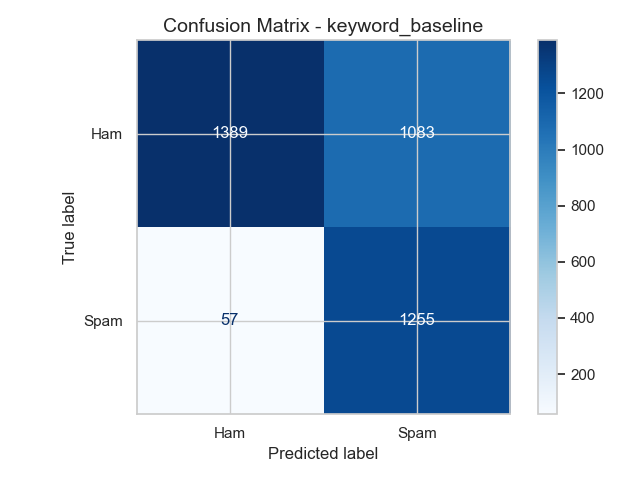
\includegraphics[width=\textwidth]{outputs/keyword_baseline_confusion_matrix.png}\\[2pt]
{\scriptsize Keyword Baseline}

\column{0.24\textwidth}
\centering
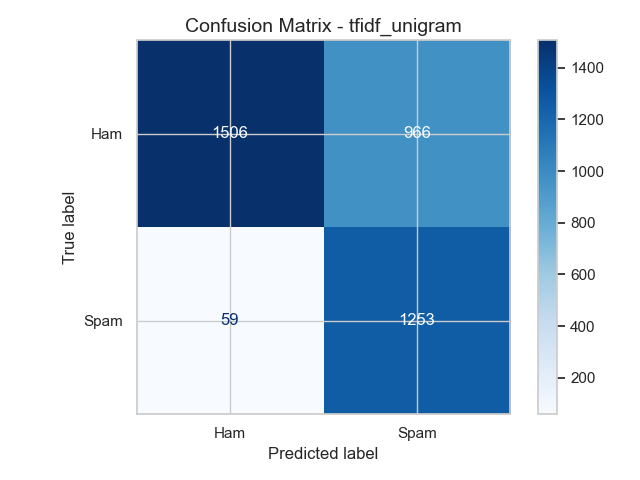
\includegraphics[width=\textwidth]{outputs/tfidf_unigram_confusion_matrix.png}\\[2pt]
{\scriptsize TF-IDF Unigram}

\column{0.24\textwidth}
\centering
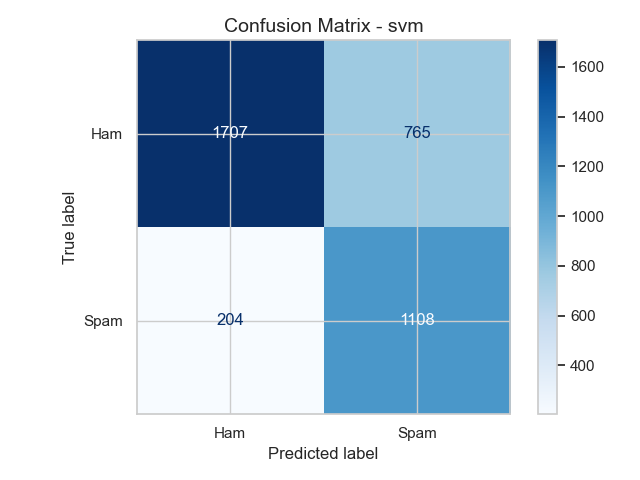
\includegraphics[width=\textwidth]{outputs/svm_confusion_matrix.png}\\[2pt]
{\scriptsize Linear SVM}

\column{0.24\textwidth}
\centering
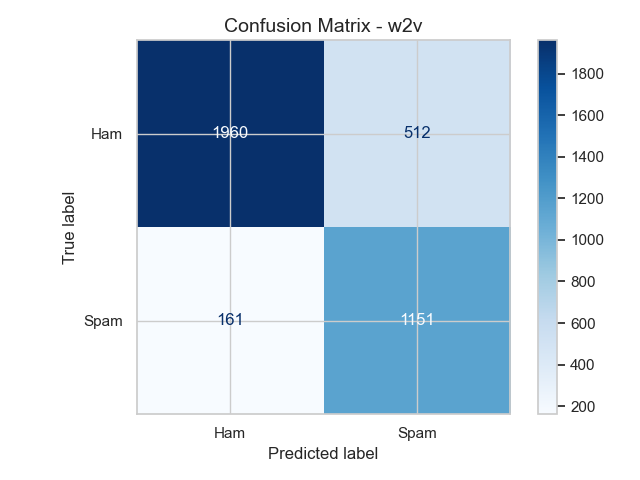
\includegraphics[width=\textwidth]{outputs/w2v_confusion_matrix.png}\\[2pt]
{\scriptsize\textcolor{accentGreen}{Word2Vec + Struct}}
\end{columns}

\vspace{10pt}
\centering
{\small From \textcolor{accentRed}{zero spam detection} at milestone $\rightarrow$ \textcolor{accentGreen}{81\% accuracy} with Word2Vec}
\end{frame}

% ============================================================
%  PERSON 5 — PR Curves
% ============================================================
\begin{frame}{Precision-Recall Curves}
\begin{columns}[c]
\column{0.32\textwidth}
\centering
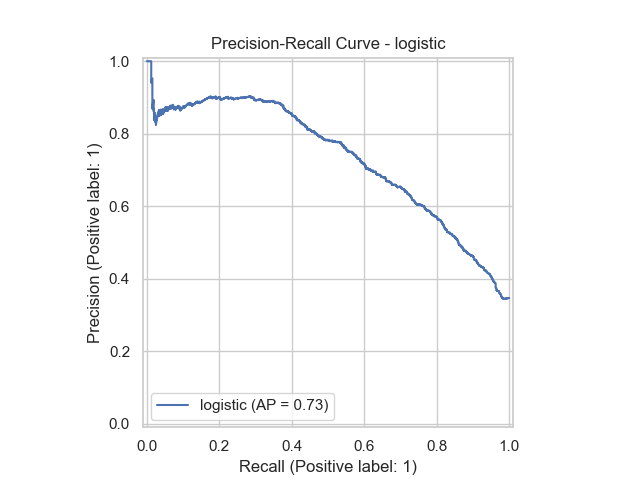
\includegraphics[width=\textwidth]{outputs/logistic_pr_curve.png}\\[2pt]
{\scriptsize Logistic (Bigram+Struct)}

\column{0.32\textwidth}
\centering
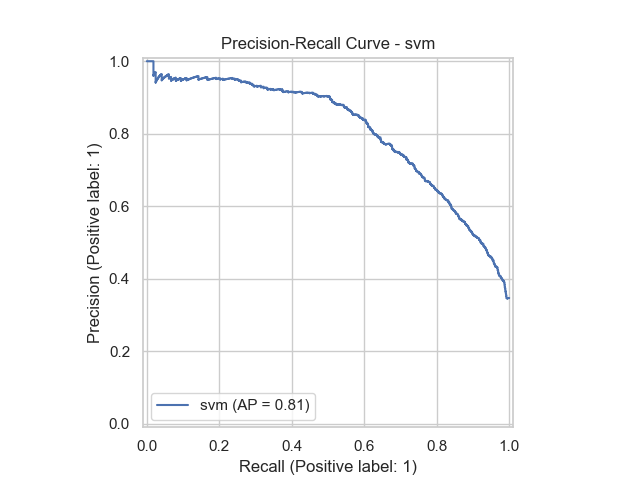
\includegraphics[width=\textwidth]{outputs/svm_pr_curve.png}\\[2pt]
{\scriptsize Linear SVM (Bigram+Struct)}

\column{0.32\textwidth}
\centering
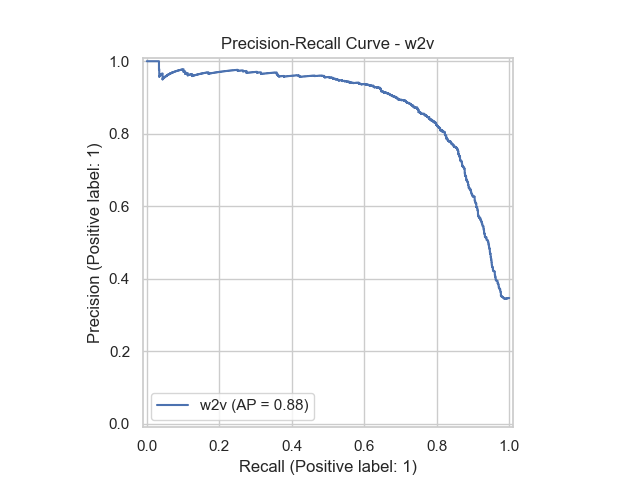
\includegraphics[width=\textwidth]{outputs/w2v_pr_curve.png}\\[2pt]
{\scriptsize\textcolor{accentGreen}{Word2Vec + Structural}}
\end{columns}

\vspace{8pt}
\centering
{\small Word2Vec maintains the strongest precision across all recall levels}
\end{frame}

% ============================================================
%  PERSON 5 — Conclusion
% ============================================================
\begin{frame}{Conclusion}
\begin{columns}[T]
\column{0.55\textwidth}
\begin{block}{What We Learned}
\begin{itemize}
    \item \textbf{IDF weighting} improves over raw keyword counts
    \item \textbf{Structural features} capture domain-invariant spam ``shape''
    \item \textbf{Linear SVM} handles noisy high-dimensional features better than Logistic Regression
    \item \textbf{Dense embeddings} (Word2Vec) bridge the vocabulary gap most effectively
\end{itemize}
\end{block}

\column{0.42\textwidth}
\begin{exampleblock}{Best Model}
\centering
\large\textcolor{accentGreen}{\textbf{Word2Vec + Structural}}\\[6pt]
\normalsize
81.21\% Accuracy\\
0.76 F1-Score\\[6pt]
{\small Dense semantic representations + explicit structural analysis}
\end{exampleblock}

\vspace{6pt}
\begin{block}{\small Future Work}
\scriptsize
\begin{itemize}
    \item Multi-class: Real / Phishing / Promo
    \item Transformer-based embeddings
    \item Real-time filtering deployment
\end{itemize}
\end{block}
\end{columns}
\end{frame}

% ============================================================
%  THANK YOU / Q&A
% ============================================================
{
\setbeamertemplate{footline}{}
\begin{frame}[plain]
\vfill
\centering
{\usebeamerfont{title}\usebeamercolor[fg]{title} Thank You!}

\vspace{16pt}
{\large\color{textLight} Questions?}

\vspace{24pt}
{\small\color{textMuted}
Nathan Xie $\cdot$ Vijwal Akula $\cdot$ Kangyi Jiang $\cdot$ Zaid Khan Mohammed $\cdot$ Brian Cochran\\[6pt]
CS 410 --- Team 18 --- Spring 2026}
\vfill
\end{frame}
}

\end{document}
